\section{System Design}\label{sec:design}

We focus on issues surrounding the protection of the runtime stack, and therefore we make the following assumptions: (i) flash memory and registers are not affected by SEUs. (ii) only one SEU will occur during a given function execution. It is rare for more than one bit to be upset simultaneously; this occurs in only 5 to 6 percent of bit flip errors~\cite{underwood1992sramorbit}. 

Our approach is designed to align with the NASA coding standards for C applied in space projects~\cite{nasa_coding_standard}. First, dynamic memory allocation is not allowed, so the heap section in RAM is not used. However, for the sake of completeness, we consider the possibility of a non-empty heap in our approach. Second, the \texttt{goto} statement is also not allowed. Finally, each function should have fewer than 60 lines of code, making the execution time of each function relatively short.

Our approach protects the system stack by introducing auxiliary assembly code. The new code is injected at both the beginning and end of each function and handles CRC calculation, CRC comparison, and memory duplication. When a function is called, the code injected at the beginning of the call calculates the CRC of the caller's stack frame and saves both the CRC and the stack frame. Before the callee returns, the code injected at the end of the function calculates the CRC of the caller's stack frame again, compares it with the saved CRC, and restores the caller's stack frame if the CRCs do not match. Since interrupts are basically special functions, we emphasize functions to demonstrate our approach.

The ASM Handler, written in Java, performs the code injection. First, the input C code is compiled to assembly using GCC. The ASM Handler then injects the assembly code. Finally, the modified code is assembled and linked into an AVR executable. In this section, we discuss the supporting memory sections, the code segments injected into the target program, the architecture of the ASM Handler, and the function execution process after code injection.

\subsection{Supporting Memory Sections}\label{sec:memory_sections}

\begin{figure}
\centering
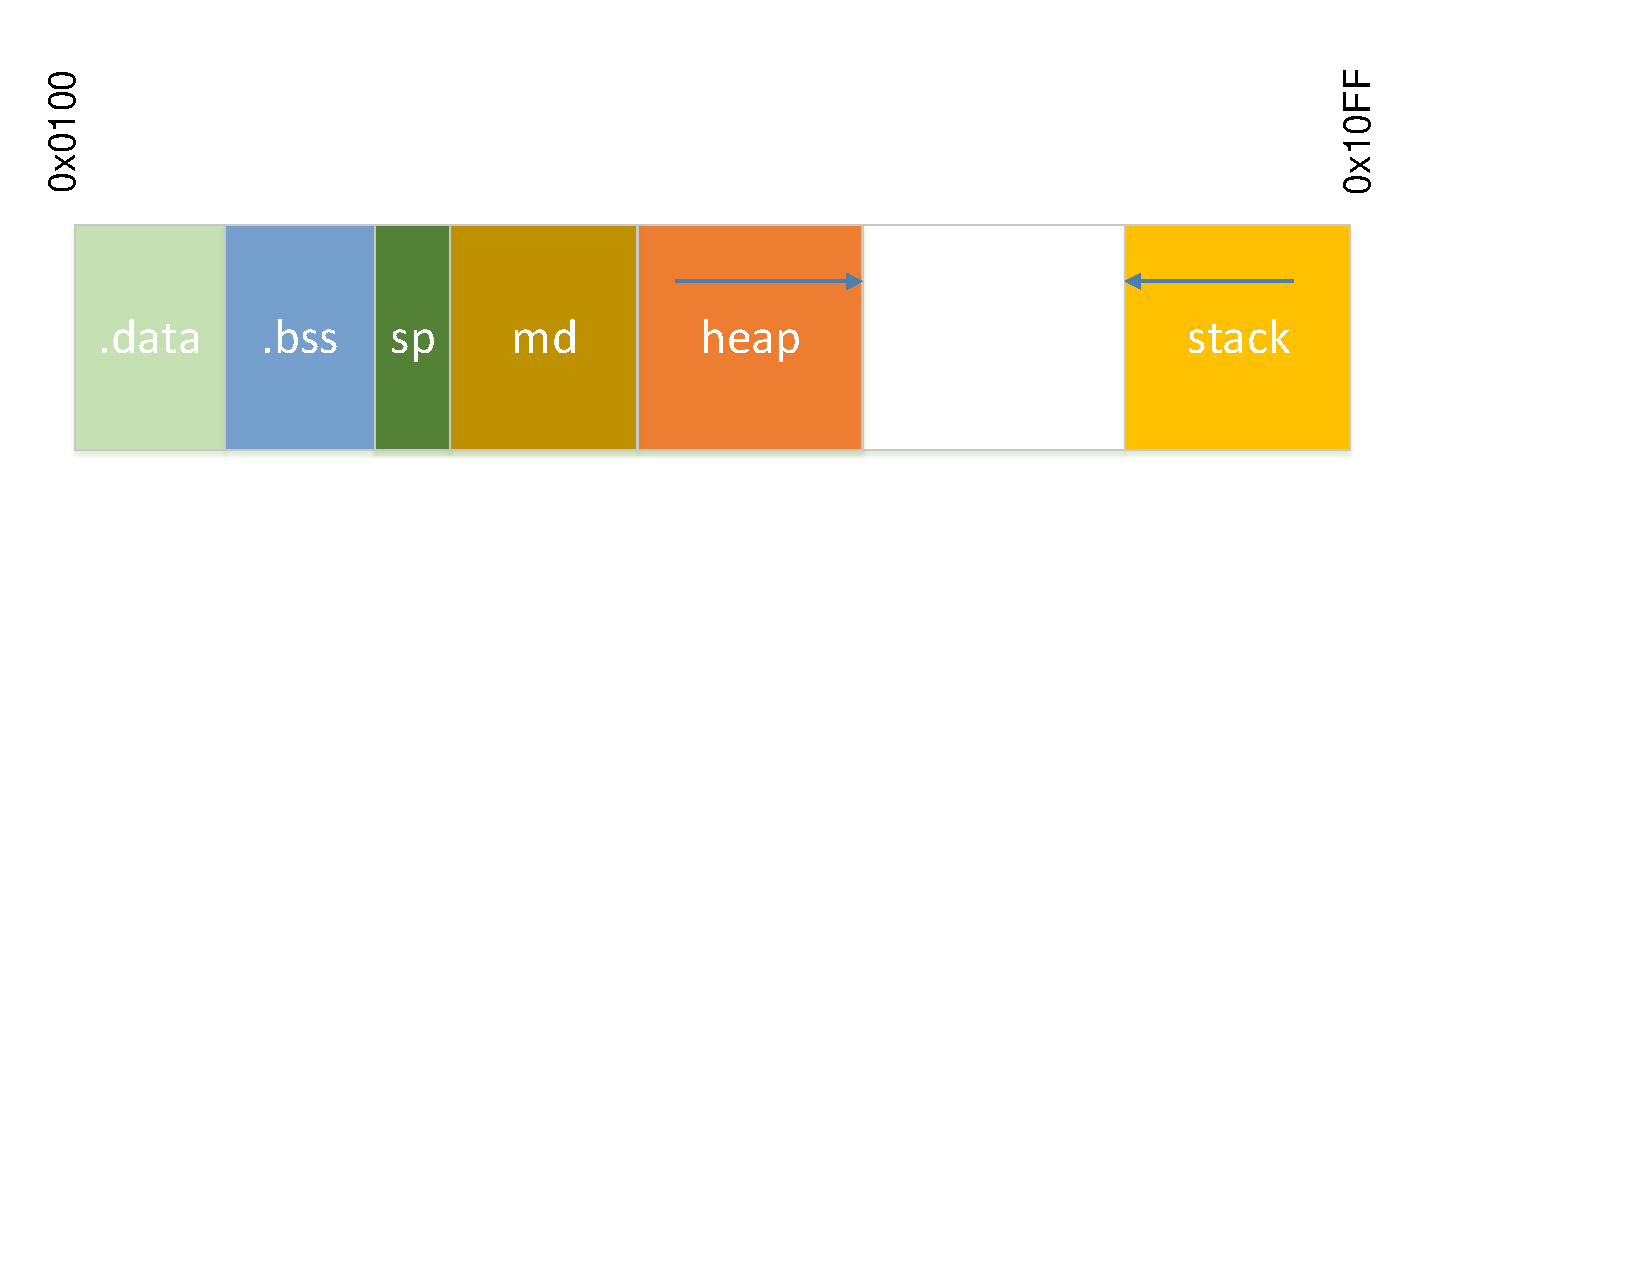
\includegraphics[scale=0.35]{figures/modified_memory_model.pdf}
\vspace{5pt}
\caption{Modified Memory Sections}
\label{fig:modified_ram_map}
\end{figure}

To store the duplicate stack frames, two new sections are created in SRAM as shown in Figure \ref{fig:modified_ram_map}, just after the \texttt{.bss} section by modifying the linker script~\cite{linkerscript}. 

The \texttt{md} section is used to store duplicate stack frames. These duplicate frames are referred to as \textit{Stack Frame Snapshots} (SFSs). The heap section grows towards the stack, and of course, the runtime usage of the heap and the stack are unpredictable. To prevent the \texttt{md} and \texttt{heap} sections from colliding, the size of the \texttt{md} section is fixed. If the heap is used, the size of the \texttt{md} section is set to 1/3 of the available space; otherwise, it is set to 1/2 of the available space. For example, if the \texttt{.data} and \texttt{.bss} sections require 1 KB in a 4 KB RAM, the space available is 3 KB, so the size of \texttt{md} is set to 1 KB.

The \texttt{sp} section is used to store the address of the next available memory space in \texttt{md}, similar to the stack pointer. This address is referred to as the \textit{Snapshot Top Pointer} (STP). To protect the STP from SEUs, the size of the \texttt{sp} section is set to 6 bytes, and 3 STP duplicates are stored in this section. Given that we assume only one SEU will occur during the execution of a given function, only one STP duplicate could be altered by a flipped bit. The altered STP is easily identified and corrected by comparing the values of the three STP duplicates.

\subsection{Injected Code Segments}

We categorize the injected code based on function. Each continuous assembly segment performs a set of operations, handling a specific action. These segments are designed to use only registers, reducing their dependency on RAM. Each segment is assigned a unique ID. Here we summarize each type of code segment.

\begin{itemize} \itemsep 0in

\item The \textit{CRC Calculation} segment (ID: CC) is used to calculate the CRC checksum of a given memory region, e.g., a stack frame. In our implementation, CRC16-CCITT is used~\cite{crc16}.

\item The \textit{CRC Save} segment (ID: CS) is used to save the CRC checksum to the stack.

\item The \textit{CRC Compare} segment (ID: CM) is used to compare two CRC checksums. The comparison result indicates whether an SEU is detected.

\item The \textit{Frame Copy} segment (ID: FC) is used to copy a stack frame to a given destination, and to save and restore stack frames.

\item The \textit{Frame Size Save} segment (ID: FS) is used to save the size of the stack frame for the current function; this will be discussed in Section \ref{sec:scanner}.

\item The \textit{STP Initialization} segment (ID: SN) is used to initialize the STP so it points to the lowest address of the \texttt{md} section.

\item The \textit{STP Update} segment (ID: SU) is used to update the STP. First, it obtains the correct STP value by comparing the three copies of the STP. Next, all three copies are updated. The segment increases the STP to save a stack frame in the SFS and decreases the STP to release a stack frame from the SFS.

\end{itemize}

\subsection{The ASM Handler}

\begin{comment}
\begin{figure*}[t]
\centering
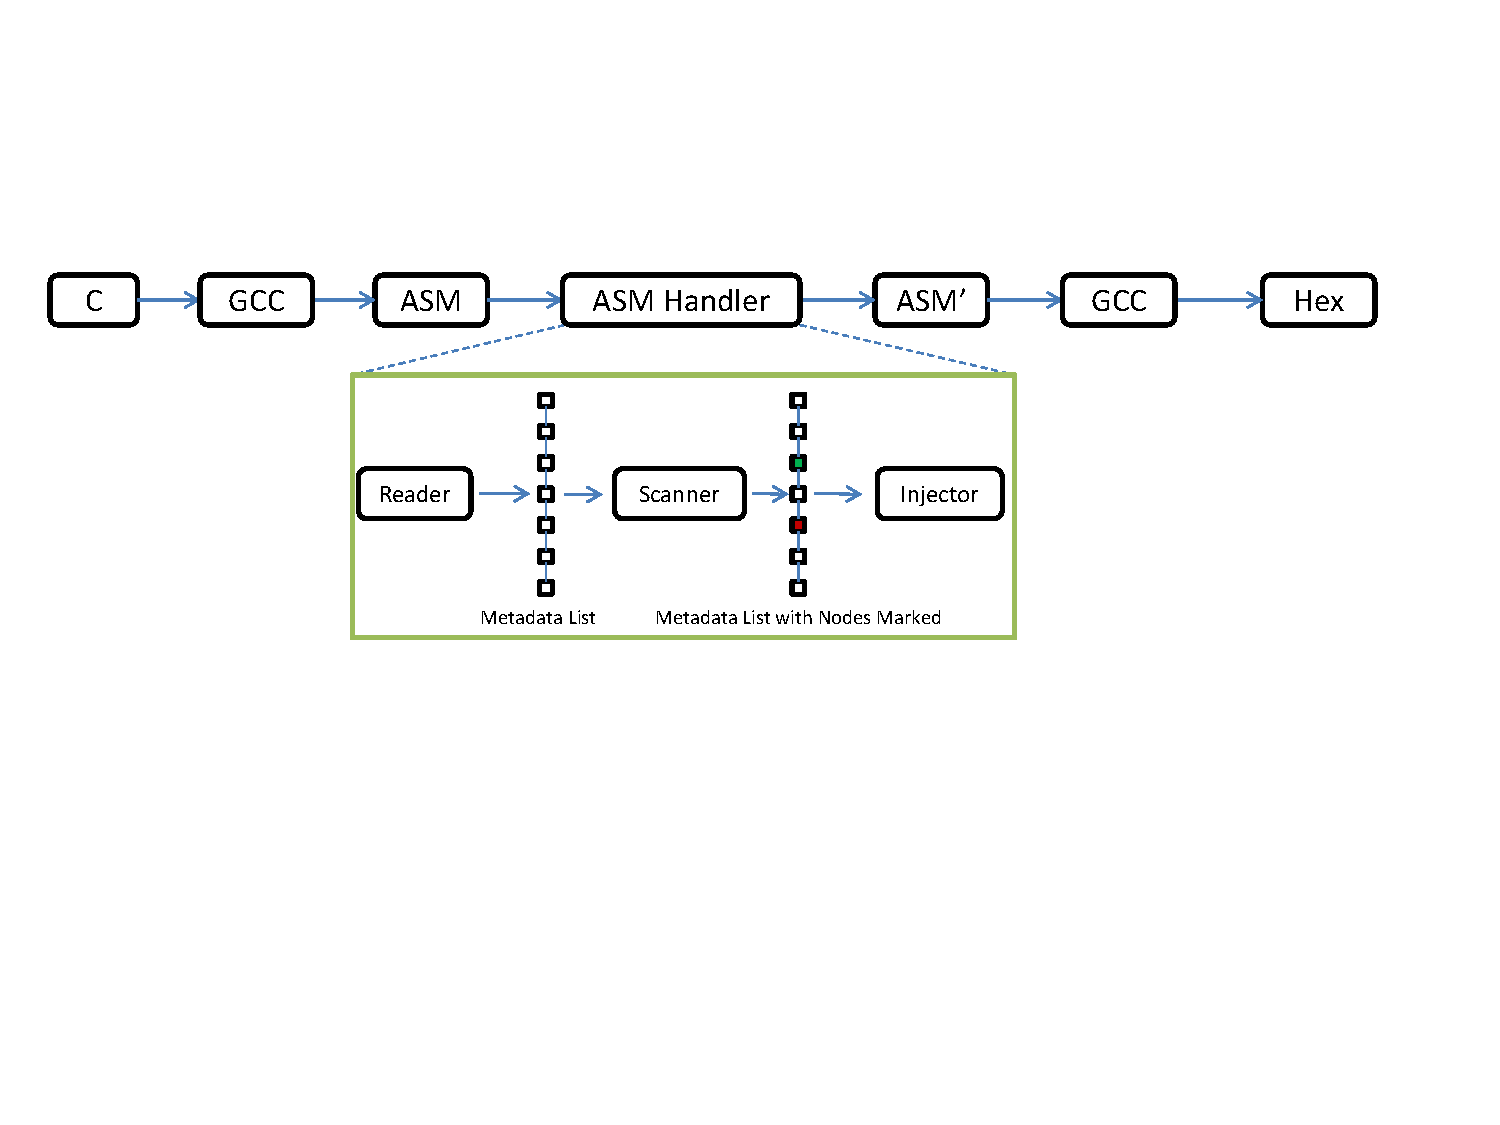
\includegraphics[width=1\textwidth]{figures/code_inject_process_v6}
\caption{Code Injection Process}
\label{fig:code_injection_process}
\end{figure*}
\end{comment}

The ASM Handler is responsible for code injection. It consists of three loosely-coupled modules: the Reader, the Scanner, and the Injector. Assembly metadata is generated to assist the code injection process. Here we describe the metadata creation process and describe each module of the ASM Handler.

\subsubsection{ASM Metadata}

Each line of assembly code is tagged with metadata representing the line of code. The metadata annotation classifies each line into one of three categories, as shown in Listing \ref{lst:metadata_example}. A \textit{directive} is used to specify assembly code information, such as the system architecture (line 1) and section (line 2), a label declaration (line 3), the label type (line 4), and other information. A \textit{label} is used to identify a location in the assembly code (line 5). In this example, \texttt{main} specifies the starting address of the main function. An \textit{instruction} is used to identify an instruction that will be executed by the microprocessor (lines 6-8). The metadata also stores code injection information, which specifies whether code is injected before or after a given line, as well as the type of code to be injected.

\begin{lstlisting}[float=tb,label=lst:metadata_example,caption=Assembly Code Example]
.arch atmega644					% directive
	.text								% directive
.global	main						% directive
	.type	main, @function		% directive
main:									% label
	push r28							% instruction
	push r29							% instruction
	...
\end{lstlisting}

\subsubsection{Reader}

The Reader is used to read the assembly file and generate corresponding metadata. It reads each line of assembly and generates a corresponding metadata node (in memory), which is then appended to a metadata list. For example, the Reader generates a list with 7 nodes after it reads the code in Listing \ref{lst:metadata_example}.%, as shown in Figure \ref{fig:code_injection_process}.

\subsubsection{Scanner}\label{sec:scanner}

The Scanner is used to scan the metadata list and mark each metadata node based on the operations performed by the associated code. Marked metadata nodes indicate that code segments will be injected either before or after the corresponding line of code.

We analyze the assembly code to identify the key operations where code segments must be injected. Here we summarize the key operations.

\begin{itemize} \itemsep 0in
\item The \textit{Stack Frame Establishment} operation is used to establish the stack frame for the current function. This operation is identified by scanning ``\texttt{sbiw r28,\textit{n}}'', which is used to establish the stack frame.

\item The \textit{Stack Frame Pointer Save} operation is used to copy the stack frame pointer to the stack pointer. This operation is identified by scanning ``\texttt{out \_\_SP\_L\_\_,r28}'', which indicates that the required registers are ready, and the function is about to execute. 

\item The \textit{Function Return} operation is used when a function returns. This operation is identified by scanning the return instruction, ``\texttt{ret}''.
\end{itemize}

The Scanner scans each node in the metadata list, checks if the code represented by the node performs one of the key operations, and marks each such node with a list of identifiers from the set (CC, CS, CM, FC, FS, SN, SU, P), where CC, CS, CM, FC, FS, SN, SU are the IDs of the code segments to be injected, and P indicates the position of the injection (i.e., before or after the assembly line). Nodes that do not require code injection are not tagged. For example, the metadata node that represents the Function Return operation is marked with (CC, CM, FC, SU, P), indicating code segments CC, CM, FC, and SU must be injected before the associated line of code.

The Scanner also extracts two information elements from the metadata list: i) The Scanner scans the metadata list and detects if \texttt{malloc} is called in the target program, which indicates whether the \texttt{heap} section in RAM is used. This information is later used in determining the section size used to store the stack frame duplicates, as discussed in Section \ref{sec:memory_sections}. ii) The Scanner determines the size of each function's stack frame by scanning the assembly code used to establish the stack frame, ``\texttt{sbiw r28, n}'', yielding a stack frame size of $n + 10$. The \texttt{n} bytes are used to store the arguments and local variables, and the additional $10$ bytes are used to store the return address, CRC, and three copies of the stack frame size, each of which requires 2 bytes.

\subsubsection{Injector}

The Injector is used to inject code segments into the target assembly code. It again scans the metadata list. When a node is marked, the Injector injects the specified code segments at the position specified by parameter $P$. Finally, a modified assembly file is generated, which is then assembled and linked to form an executable file.

In our initial approach, the code segments were directly injected into the target code, effectively making the code segments \textit{inlined}. The results showed that the ROM overhead was significant. Each function, regardless of its size, was injected with code segments that require approximately 500 bytes of ROM. In our final approach, all the code segments are injected at the end of the target code, and each is labeled with its unique ID. When scanning the metadata list, instead of injecting the code segments into the target code, a function call instruction, \texttt{call}, is injected. A function return instruction, \texttt{ret}, is added at the end of each code segment. Because each segment was designed to use only registers, only two stack bytes are needed by each segment to save the return address. We discuss the performance of both approaches in Section \ref{sec:evaluation}.

\subsection{Modified Function Execution Process}

The auxiliary code injected at the beginning and end of each function modifies the function execution process, including the invocation sub-process and the return sub-process. Below is a description of the modified processes.

\subsubsection{Modified Function Invocation Process}

The code segments injected at the beginning of each function are used to calculate a CRC over the caller's stack frame, and to save a duplicate of the caller's stack frame, as shown in Figure \ref{fig:modified_function_operation_pre_execution}. Figure \ref{fig:modified_function_operation_process_pre_execution} shows the execution process of the pre-invocation code; Figure \ref{fig:modified_function_operation_stack_pre_execution} shows the stack changes associated with the pre-invocation code. Each rectangle represents two stack bytes. In the execution process diagram, the white ovals denote operations performed by the original code, and the shaded ovals denote operations performed by the injected code. In the stack diagram, \texttt{SP} denotes the stack pointer, and \texttt{Y} denotes the stack frame pointer. As before, the numbers below each stack identify the operations that changed the stack.

When a function \texttt{B} is called by a function \texttt{A}, the return address is pushed onto the stack automatically by the function call instruction (step 1). To calculate the CRC of the caller's stack frame, multiple registers are used, so they must be saved before the CRC calculation process, and restored when the process is finished. To prevent the calculated CRC from being overwritten when the registers are restored, two bytes are pushed onto the stack as a placeholder (step 2) for the CRC result before the registers used to calculate the CRC are saved (step 3). After the CRC of function \texttt{A}'s stack frame is calculated (step 4), the CRC result is saved to the placeholder location (step 5). The registers used to calculate the CRC are then restored (step 6).

Next, the stack frame of the caller, function \texttt{A}, has to be saved. The registers used to save the stack frame are pushed onto the stack (step 7). Next, the correct STP is selected by comparing the values of the three STP copies (step 8). Using the correct STP, the specified memory is then copied and saved in the SFS (step 9). After the STP copies are updated (step 10), the CRC registers are restored (step 11).

After the stack frame pointer of function \texttt{B} is saved (step 12), and the stack frame is established (step 13), three copies of the stack frame size of the callee, function \texttt{B}, are pushed onto the stack (step 14), which is a key operation in the injected code. 

When a function is called, the return address is pushed onto the stack, and later used when the function returns. However, the callee does not have sufficient context regarding its caller, including the caller's stack frame address and size. It is impossible for the callee to calculate the CRC of the caller's stack frame and to duplicate the stack frame without this information. To solve this problem, each function saves its stack frame size in the stack, which is used by its callee to perform the CRC calculation and stack frame copy. To ensure the correctness of the stack frame size, three copies are saved. Comparison is used to yield the correct value. 

\begin{figure}[h]
        \centering
        \begin{subfigure}[b]{0.4\columnwidth}
                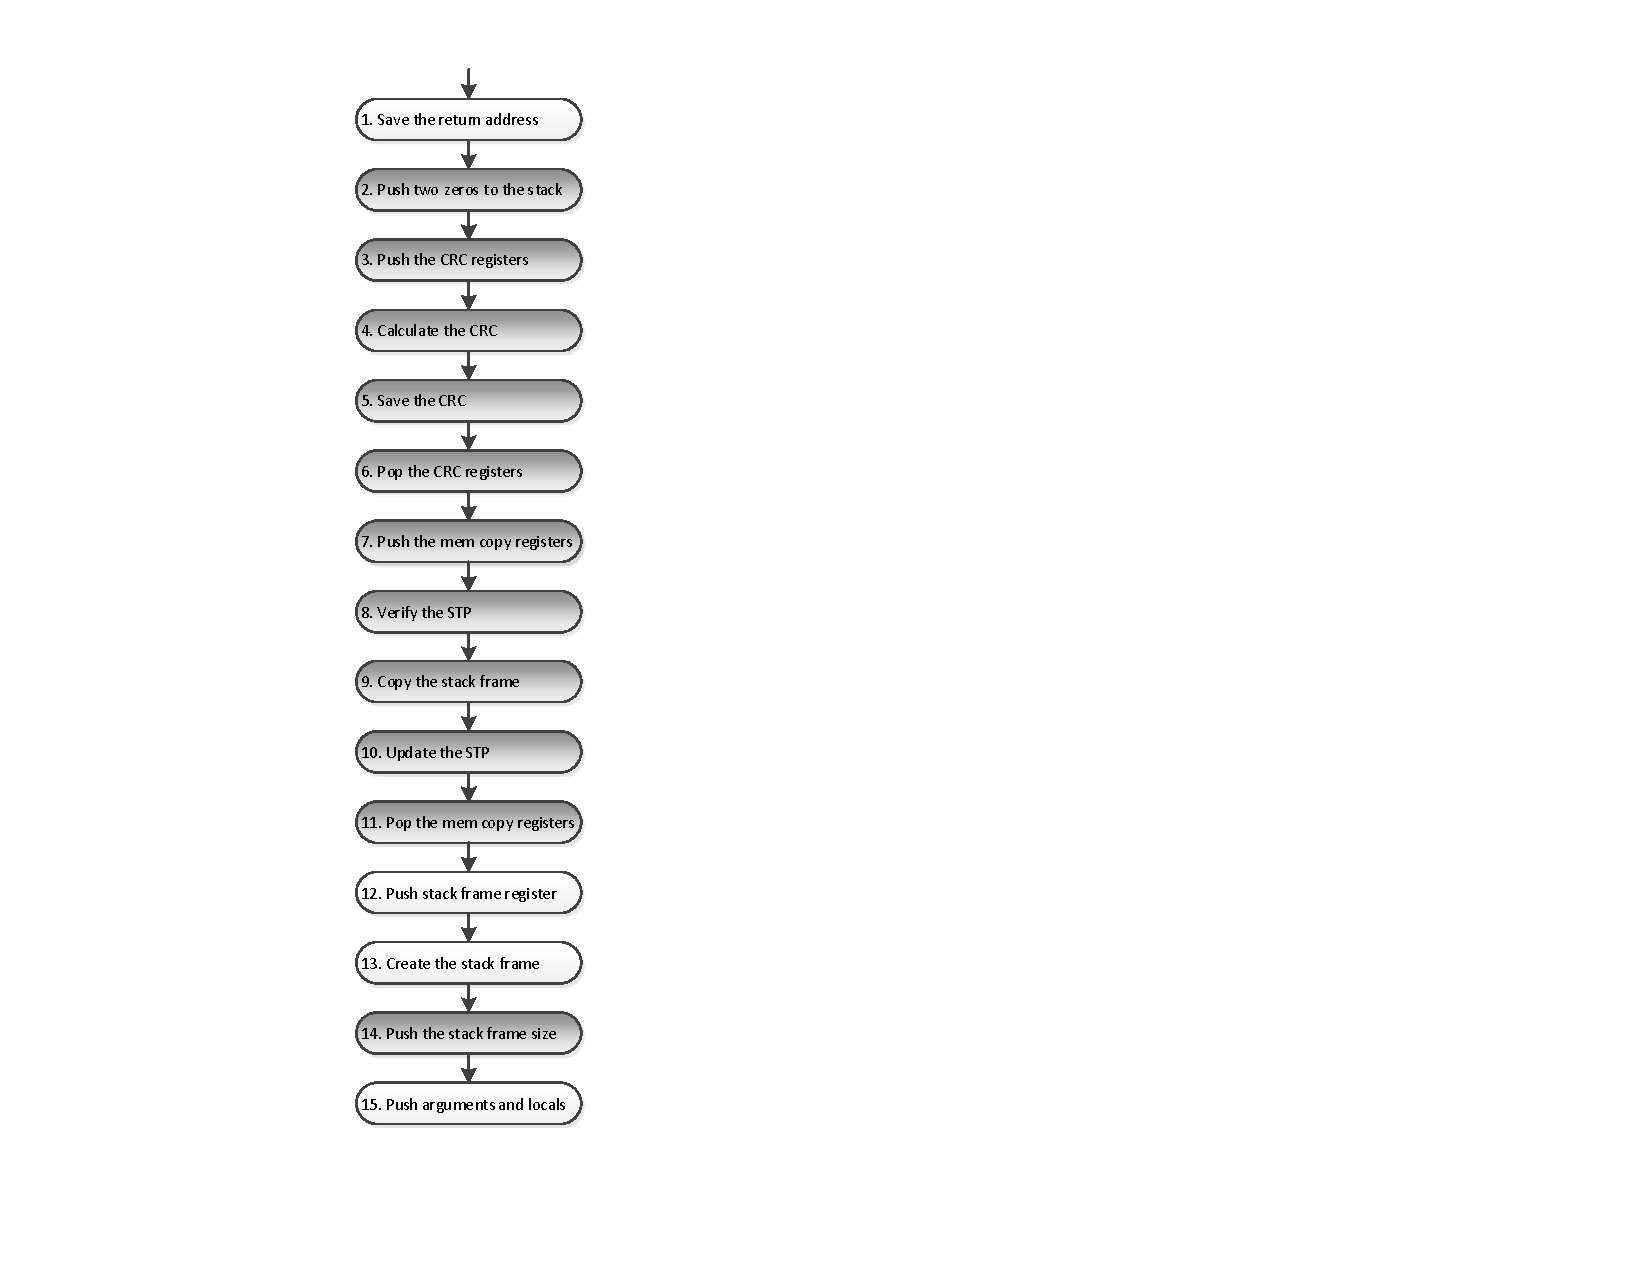
\includegraphics[width=\textwidth, height=12cm]{figures/modified_function_operations_process_pre_execution_v2}
                \caption{Process}
                \label{fig:modified_function_operation_process_pre_execution}
        \end{subfigure}~
        \begin{subfigure}[b]{0.6\columnwidth}
                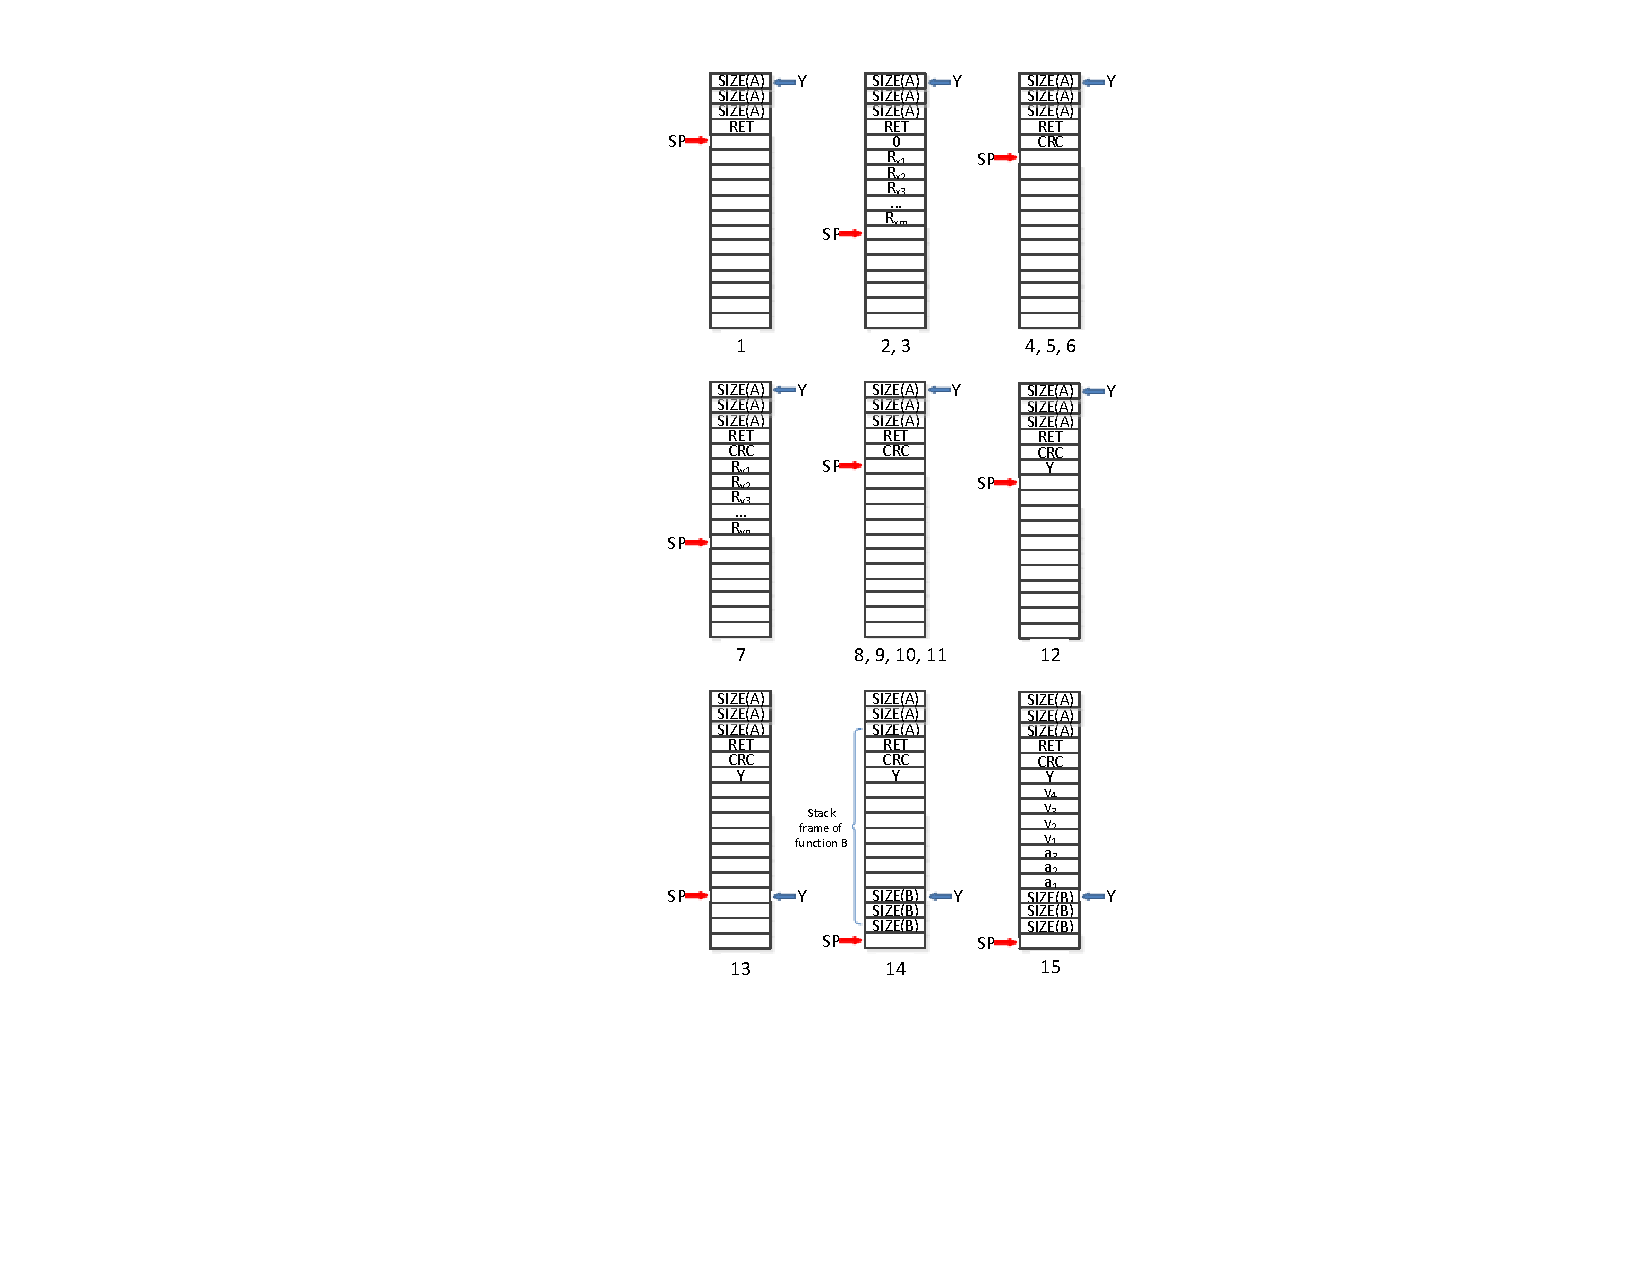
\includegraphics[width=\textwidth, height=12cm]{figures/modified_function_operations_stack_pre_execution_v2}
                \caption{Stack}
                \label{fig:modified_function_operation_stack_pre_execution}
        \end{subfigure}
		\vspace{10pt}
        \caption{Modified Function Invocation Process}\label{fig:modified_function_operation_pre_execution}
\end{figure}

\subsubsection{Modified Function Return Process}

The code segments injected at the end of each function are used to verify the stack frame of the caller function, and to restore the stack frame if an SEU is detected, as shown in Figure \ref{fig:modified_function_operation_post_execution}. Each rectangle represents two stack bytes. Again, in the execution process diagram, the white ovals denote operations performed by the original code, and the shaded ovals denote operations performed by the injected code.

When function \texttt{B} returns, it first pops its stack frame size (step 1). After the space used to store the arguments and local variables is released (step 2), the stack frame pointer is restored (step 3). The CRC of function \texttt{A}'s stack frame is then calculated and temporarily stored in two registers (steps 4-6). The values stored in these registers are saved before the function return process. Next, the calculated CRC is compared with the CRC saved in the stack (step 7). If the two CRCs do not match, the saved stack frame of \texttt{A} is restored, and the STP is updated to release the space used to store the stack frame of \texttt{A} (steps 8-12). Again, the stack frame size of function \texttt{A} saved in the stack is used to support the CRC comparison and stack frame restoration (if needed). If the two CRCs match, the STP is updated (steps 13-14). After verification of \texttt{A}'s stack frame is complete, the CRC is popped from the stack (step 15). Finally, function \texttt{B} returns, and the return address is popped automatically (step 16).

\begin{figure}[h]
        \centering
        \begin{subfigure}[b]{0.5\columnwidth}
                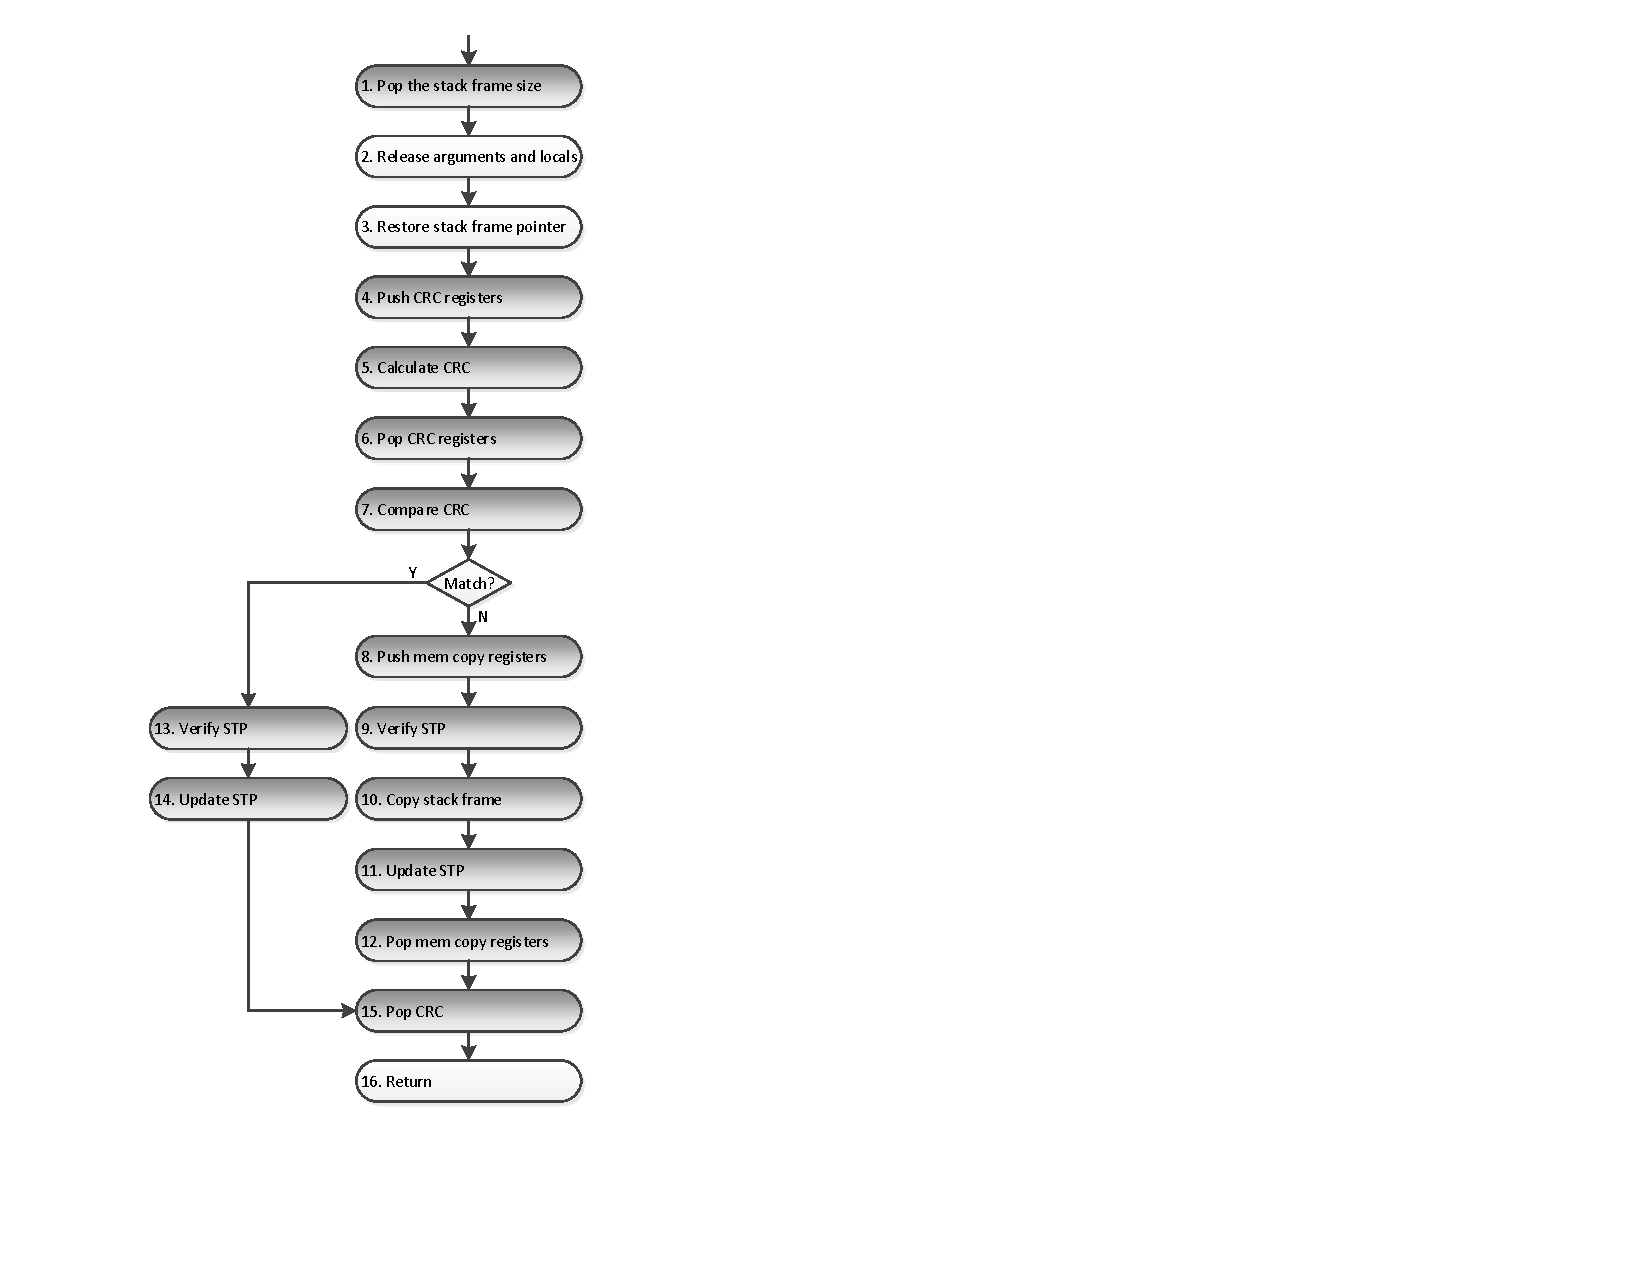
\includegraphics[width=\textwidth, height=12cm]{figures/modified_function_operations_process_post_execution_v2}
                \caption{Process}
                \label{fig:modified_function_operation_process_post_execution}
        \end{subfigure}~
        \begin{subfigure}[b]{0.5\columnwidth}
                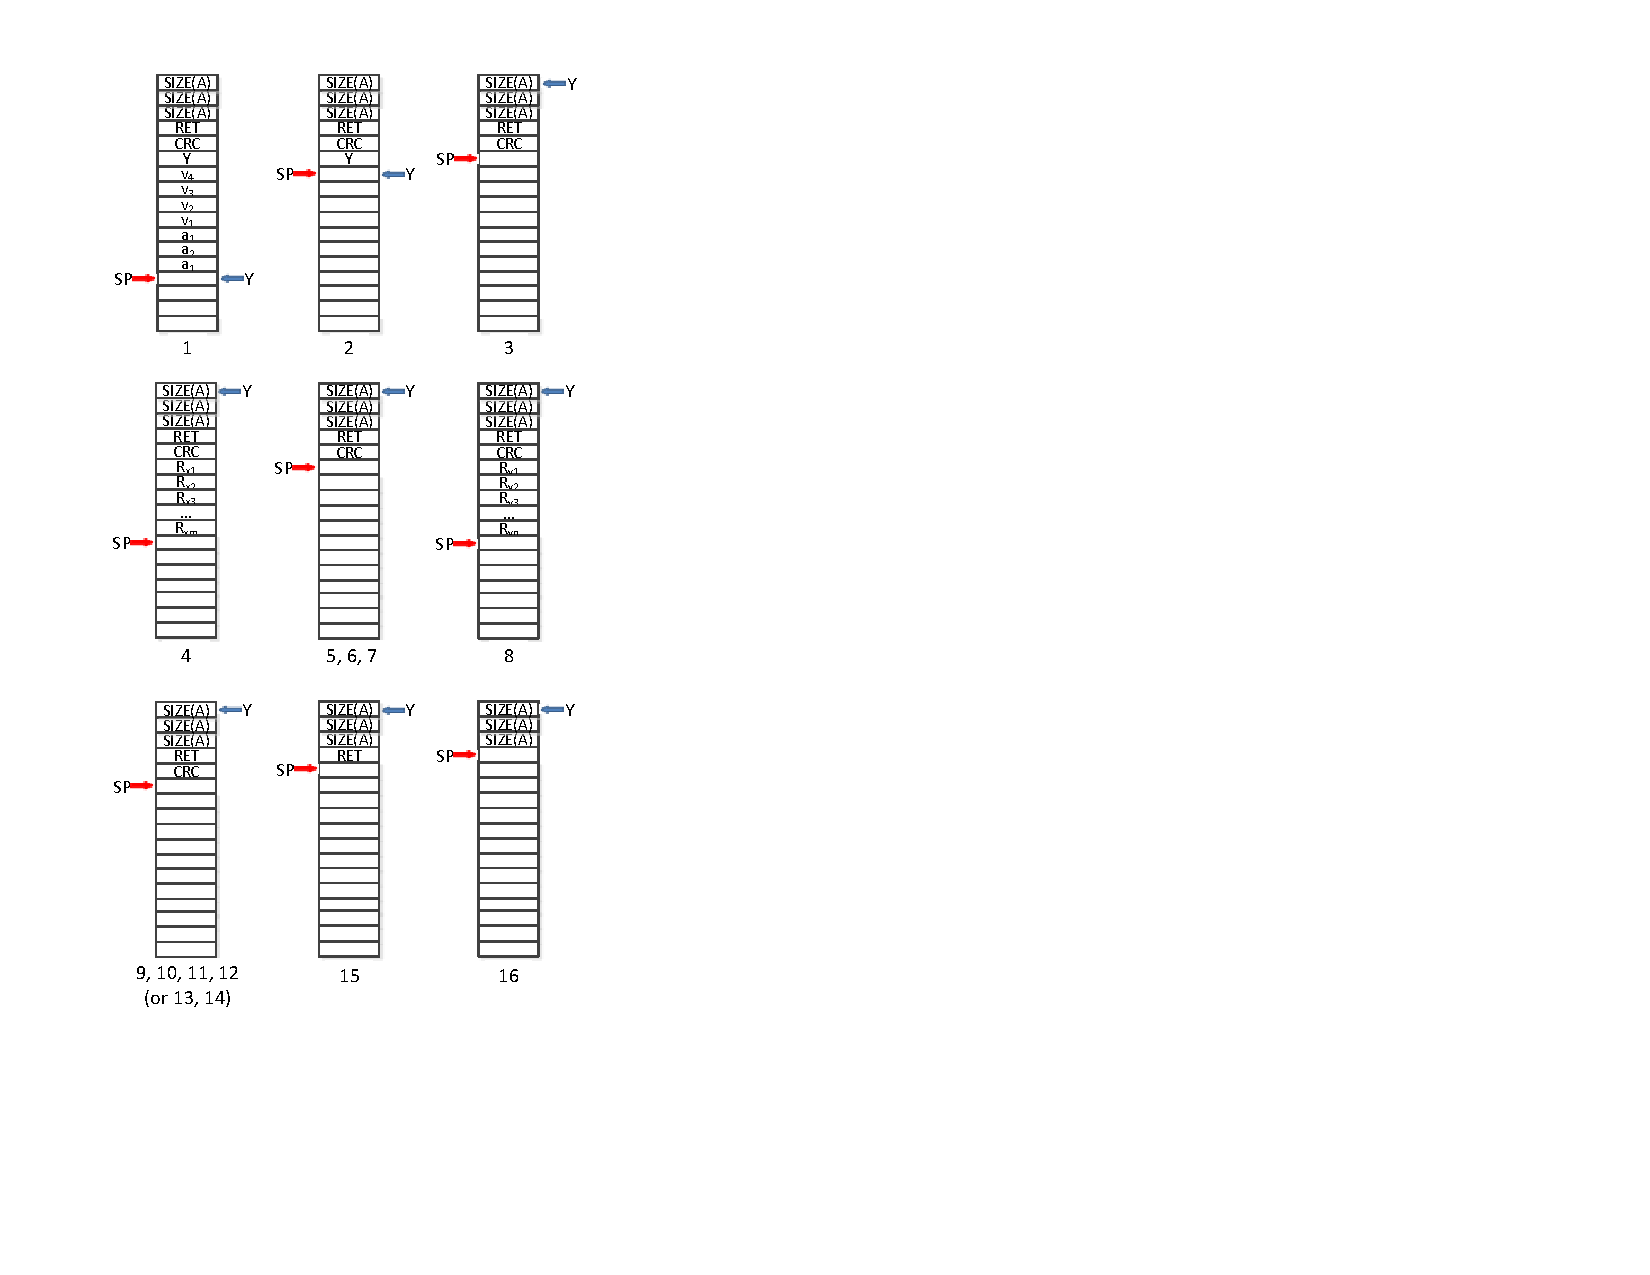
\includegraphics[width=\textwidth, height=12cm]{figures/modified_function_operations_stack_post_execution_v2}
                \caption{Stack}
                \label{fig:modified_function_operation_stack_post_execution}
        \end{subfigure}
        \vspace{10pt}
        \caption{Modified Function Return Process}\label{fig:modified_function_operation_post_execution}
\end{figure}
